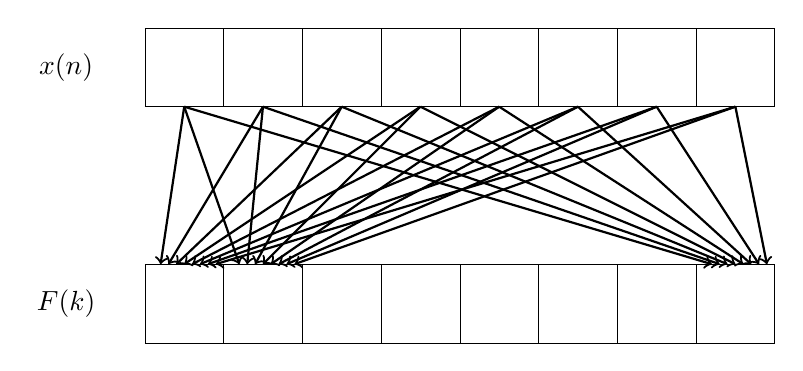
\begin{tikzpicture}[level/.style={sibling distance=60mm/#1}]

\node at (-5,1.5) {$x(n)$};
\node at (-5,-1.5) {$F(k)$};

\draw[step=1cm,very thin] (-4,-2) grid (4,-1);

\draw[step=1cm,very thin] (-4,1) grid (4,2);

\visible<1>{
\foreach \s in {0,...,7}{
    \draw[thick,->] (-3.5+\s,1) -- (-3.8+\s*0.1,-1);
}
}

\visible<2>{
\foreach \s in {0,...,7}{
    \draw[thick,->] (-3.5+\s,1) -- (-2.8+\s*0.1,-1);
}
}

\visible<3>{
\foreach \s in {0,...,7}{
    \draw[thick,->] (-3.5+\s,1) -- (3.2+\s*0.1,-1);
}
}


\end{tikzpicture}
